\section*{\textbf{7 - Building a quadtree} \hrule} 



\subsection*{\textbf{Question 7}}
\begin{quote}

\textbf{Problem}
\begin{quote}
Download the file containing 1200 particle masses and positions. Considering only the x and y coordinates of these particles (between 0 and 150), construct a Barnes-Hut quadtree with at most 12 particles per leaf node. You can treat the masses and positions as dimensionless and use $G = 1$. Plot the particles and indicate which particles are in which node. Calculate the $n = 0$ multipole moment of each leaf and then recursively for each node in the tree. Print the $n = 0$ mulitpole moment for the leaf node containing the particle with index $i = 100$ and that of all its parent nodes up to and including the root node.
\end{quote}

\textbf{Solution} 
\begin{quote}
The zeroth order multipole moment for a leaf node corresponds to the sum of the masses of the particles in that leaf node. The multipole moment of a parent node (can be a parent of a leaf, or of a other non leaf) is the sum of the multipole moment of its children. With this knowledge a quadtree has been constructed that calculates the multipole moment for each of its nodes. The origin of the tree is chosen to be x = 0, y = 0 and corresponds with the left bottom coordinate of the root quad. The size of the root node is chosen to be 150. The root node is thus a quad with edge points: (0,0) (origin), (150,0) right bottom, (0,150) left top, (150,150) right top. 
\\
The code for the tree, a plot of the particles in the tree and the multipole moments can be found below. The code is split over two files, the first file 
contains the code that constructs  the quad tree and adds the particles to the tree. The second file contains the code that contains the quad tree its self.   
\end{quote}

\textbf{Code - Output}
\begin{quote}
The code that constructs the quad tree and adds the particles to it.
\lstinputlisting{./Code/assigment_7.py}
\end{quote}

\textbf{Code - Tree}
\begin{quote}
The code of the quadtree.
\lstinputlisting{./Code/mathlib/quadtree.py}

\end{quote}
\textbf{Output - Text}
\begin{quote}
The text output produced by the code. This consists of the multipole moments
of the leaf containing the particle with index 100 and its parents. The first
line is thus the multipole moment of the leaf containing the particle with index 100 and the last line is the multipole moment of the root. 
\lstinputlisting{./Output/assigment7_out.txt}
\end{quote}

\textbf{Output - Plot}
\begin{quote}
\begin{figure}[!ht]
\centering
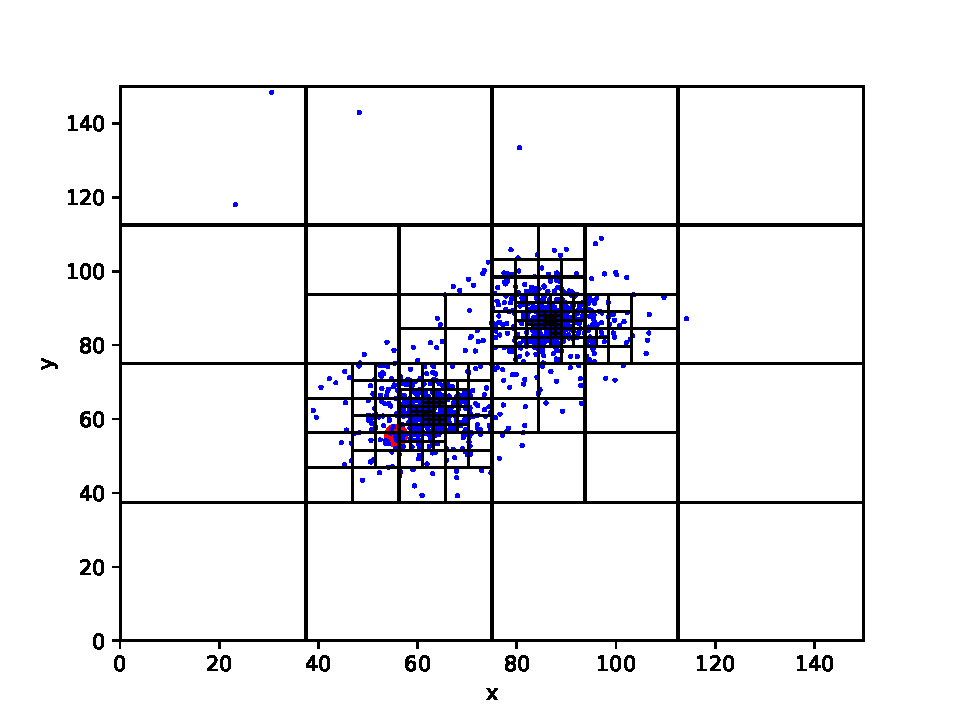
\includegraphics[width=14cm, height=8.5cm]{./Plots/7_quadtree.pdf}
\caption{A visual representation of the constructed quadtree. The blue points indicate the positions of the bodies added to the tree. The red point indicates the position of the body with index 100.}
\end{figure}
\end{quote}



\end{quote}










